\begin{frame}{Gradient Descent}
  \begin{align*}
    p(c|x) = y(x) = \sigma(Wx),~~\sigma_{i}(x) = \frac{e^{x_{i}}}{\sum_{\forall j}e^{x_{j}}}
  \end{align*}
  \begin{align*}
    \nabla E(\theta) = \sum_{i}(y_{i}-t_{i})x_{i}
  \end{align*}


  \note{
    \begin{itemize}
      \item The introduced formulation for Logistic Regression has no analytical solution.
      \item We can search for minima by walking on the error surface in the direction of steepest decent.
    \end{itemize}
  }
\end{frame}


\begin{frame}{Gradient Descent}

  \begin{columns}
    \begin{column}{0.7\textwidth}
      \begin{figure}
        \includegraphics[width=0.99\textwidth]{alps}
      \end{figure}
    \end{column}
    \begin{column}{0.28\textwidth}
      \begin{equation*}
        \nabla E(\theta) = \sum_{i}(y_{i}-t_{i})x_{i}
      \end{equation*}
    \end{column}
  \end{columns}

  \note{
    \begin{itemize}
      \item We start at a random point and search for a minimum by walking on the error surface in the direction of steepest decent.
    \end{itemize}
  }
\end{frame}

\begin{frame}{Gradient Descent}
  \begin{figure}
    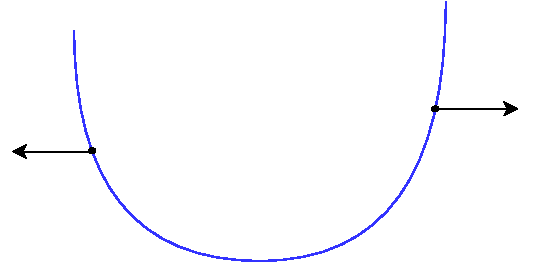
\includegraphics[width=0.8\textwidth]{gradient_descent_00}
  \end{figure}

  \note{
    \begin{itemize}
      \item For the error $E(\Theta)$ blue, the gradient points into the direction of steepest ascent.
    \end{itemize}
  }
\end{frame}


% \begin{frame}{Gradient Descent}
%   \begin{figure}
%     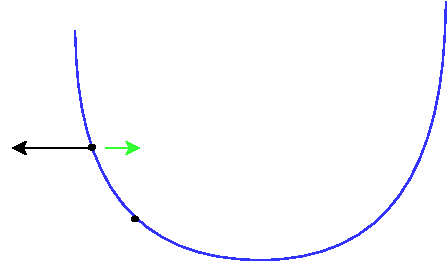
\includegraphics[width=0.75\textwidth]{gradient_descent_01a}
%   \end{figure}

%   \note{
%     \begin{itemize}
%       \item Given a random initialization for $\theta$ we can evaluate the derivative and move into opposite direction.
%     \end{itemize}
%   }
% \end{frame}


% \begin{frame}{Gradient Descent}
%   \begin{figure}
%     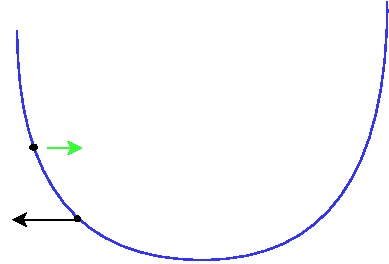
\includegraphics[width=0.75\textwidth]{gradient_descent_01b}
%   \end{figure}

%   \note{
%     \begin{itemize}
%       \item We repeat the procedure at the new $\theta$.
%     \end{itemize}
%   }
% \end{frame}


% \begin{frame}{Gradient Descent}
%   \begin{figure}
%     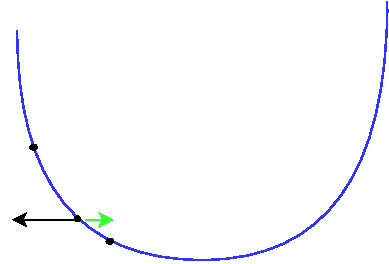
\includegraphics[width=0.75\textwidth]{gradient_descent_01c}
%   \end{figure}

%   \note{
%     \begin{itemize}
%       \item  We repeat the procedure at the new $\theta$.
%     \end{itemize}
%   }
% \end{frame}


% \begin{frame}{Gradient Descent}
%   \begin{figure}
%     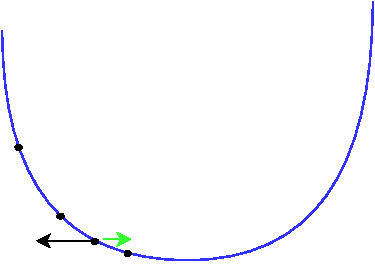
\includegraphics[width=0.75\textwidth]{gradient_descent_01d}
%   \end{figure}

%   \note{
%     \begin{itemize}
%       \item  We repeat the procedure at the new $\theta$.
%     \end{itemize}
%   }
% \end{frame}


\begin{frame}{Gradient Descent}
  \begin{figure}
    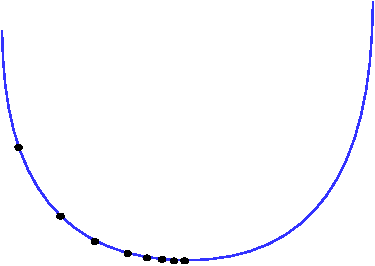
\includegraphics[width=0.75\textwidth]{gradient_descent_01e}
  \end{figure}

  \note{
    \begin{itemize}
      \item And end up at a local minimum.
    \end{itemize}
  }
\end{frame}


\begin{frame}{Gradient Descent}
  \begin{columns}
    \begin{column}{0.48\textwidth}
      \begin{figure}
        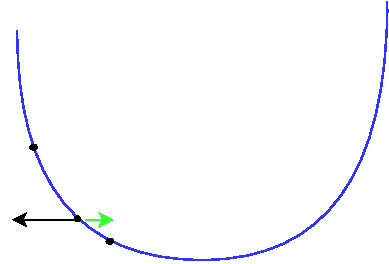
\includegraphics[width=0.9\textwidth]{gradient_descent_01c}
      \end{figure}

    \end{column}
    \begin{column}{0.48\textwidth}
      \begin{equation*}
        \theta_{i+1} = \theta_{i} - \eta \nabla E(\theta)
      \end{equation*}
    \end{column}
  \end{columns}
  \note{
    \begin{itemize}
      \item  We can write the update step formally including the learning rate (step size) $\eta$.
      \item  Whereas $\nabla$ is the gradient operator.
    \end{itemize}
  }
\end{frame}


\begin{frame}{Gradient Descent with Momentum}
  \begin{columns}
    \begin{column}{0.48\textwidth}
      \begin{equation*}
        \theta_{i+1} = \theta_{i} - \eta \nabla E(\theta)
      \end{equation*}
    \end{column}
    \begin{column}{0.48\textwidth}

      \begin{align*}
        z_{i+1} &= \beta z_{i} + \nabla E(\theta) \\
        \theta_{i+1} &= \theta_{i} - \eta z_{i+1}
      \end{align*}

    \end{column}
  \end{columns}
  \note{
    \begin{itemize}
      \item Momentum is the heavy backpack for our mountain hiker.
      \item It helps to overcome small riddles, valleys and local minima.
      \item Quadratic speedup compared to plain gradient descent on some error functions.
      \item It is a own field of research, a good starting point for the interested is maybe this article on distill: \\
            \url{https://distill.pub/2017/momentum/}
    \end{itemize}
  }
\end{frame}



\begin{frame}{Stochastic Gradient Descent}
  \begin{equation*}
    E(\theta) = \sum_{i}E_{i}(\theta)
  \end{equation*}

  \begin{equation*}
    \theta_{i+1} = \theta_{i} - \eta \nabla \sum_{j}E_{j}(\theta)
  \end{equation*}

  \note{
    \begin{itemize}
      \item The error function includes a sum over all data points.
      \item If we use all data points for the computation of the gradient (batch methods) there would be better ways of doing that than gradient descent.
      \item Furthermore, the size of the data set often would make it very expensive to use all data points.
      \item However what we usually do when training neural networks is online learning.
      \item This means we use only one sample or a subset of samples $j$ (mini-batch) at a time.
    \end{itemize}
  }
\end{frame}


% \begin{frame}{Stochastic Gradient Descent}
%   \begin{itemize}
%     \item How to choose samples? $\rightarrow$ Draw randomly without replacement.
%     \item How many samples? \\
%           $\rightarrow$ In CV often as many as possible (VRAM limiting factor) \\
%           $\rightarrow$ Higher batch size $\rightarrow$ less gradient noise $\rightarrow$ higher learning rate $\eta$
%     \item However, gradient noise allows to escape local optima! \\
%           $\rightarrow$ Too big batch sizes possible.
%   \end{itemize}

%   \note{
%     \begin{itemize}
%       \item ...
%     \end{itemize}
%   }
% \end{frame}


% \begin{frame}{Gradient Descent for Logistic Regression}
%   \begin{figure}
%     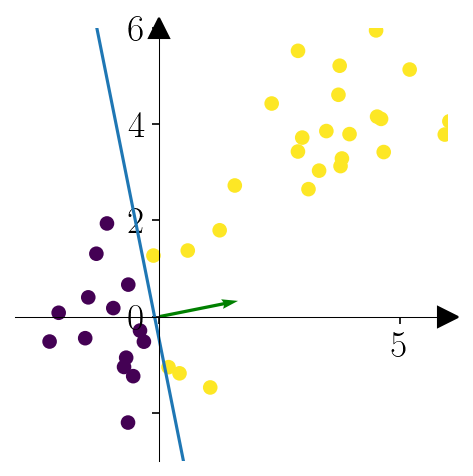
\includegraphics{gradient_descent_logistic_regression_00}
%   \end{figure}

%   \note{
%     \begin{itemize}
%       \item
%       \item
%     \end{itemize}
%   }
% \end{frame}


\begin{frame}{Gradient Descent for Logistic Regression}
  \begin{figure}
    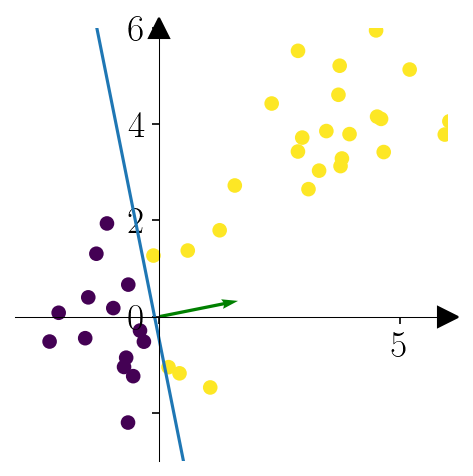
\includegraphics[width=0.3\textwidth]{gradient_descent_logistic_regression_00}
    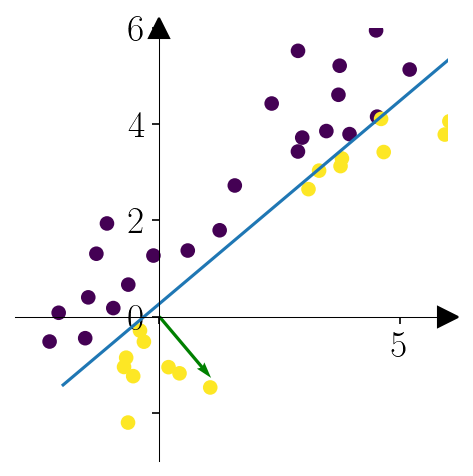
\includegraphics[width=0.3\textwidth]{gradient_descent_logistic_regression_20}
    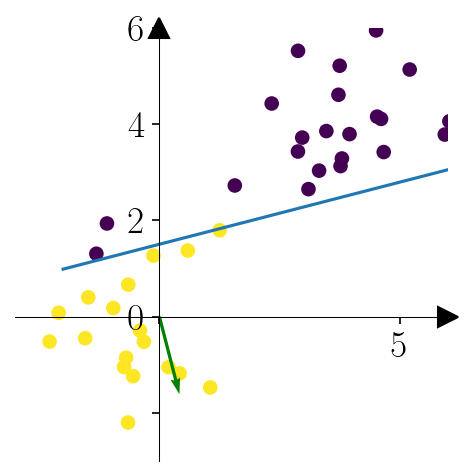
\includegraphics[width=0.3\textwidth]{gradient_descent_logistic_regression_60}\\
    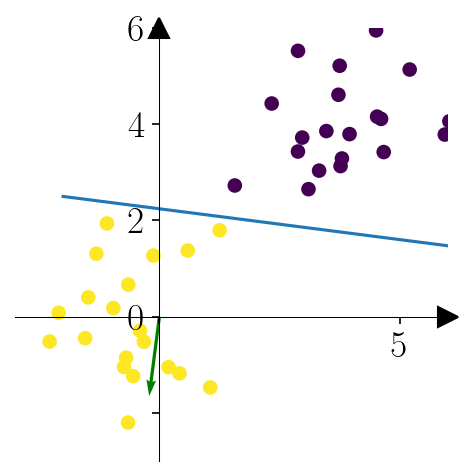
\includegraphics[width=0.3\textwidth]{gradient_descent_logistic_regression_80}
    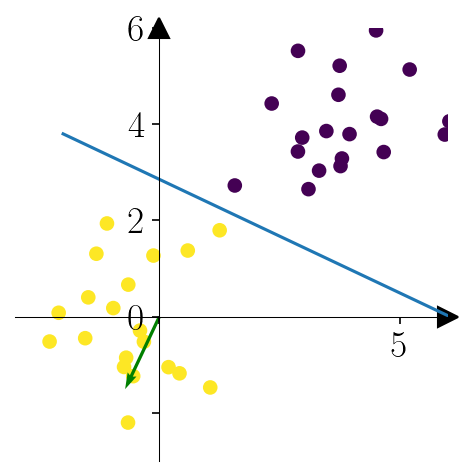
\includegraphics[width=0.3\textwidth]{gradient_descent_logistic_regression_100}
    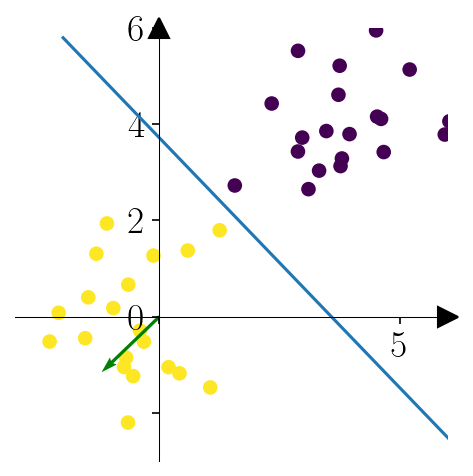
\includegraphics[width=0.3\textwidth]{gradient_descent_logistic_regression_180}
  \end{figure}

  \note{
    \begin{itemize}
      \item Progress of gradient decent optimization for linear regression.
    \end{itemize}
  }
\end{frame}
